\chapter{Produkt}
\label{chap:produkt}

Dieses Kapitel hat zum Ziel das Produkt genauer zu definieren.

\section{Need}
\label{sec:need}

\section{Approach}
\label{sec:apporach}

Im Brainstorming haben wir mehrere m�gliche L�sungswege ausgearbeitet, dieser Abschnitt zeigt drei Wege auf, w�gt sie ab und  begr�ndet den Weg den wir nehmen wollen.

\subsection{Durchfluss}
\label{ssec:durchfluss}

Der Sensor wird in der Toilette installiert und misst Feuchtigkeit oder Wasserdurchfluss.

\begin{figure}[H]
	\centering
	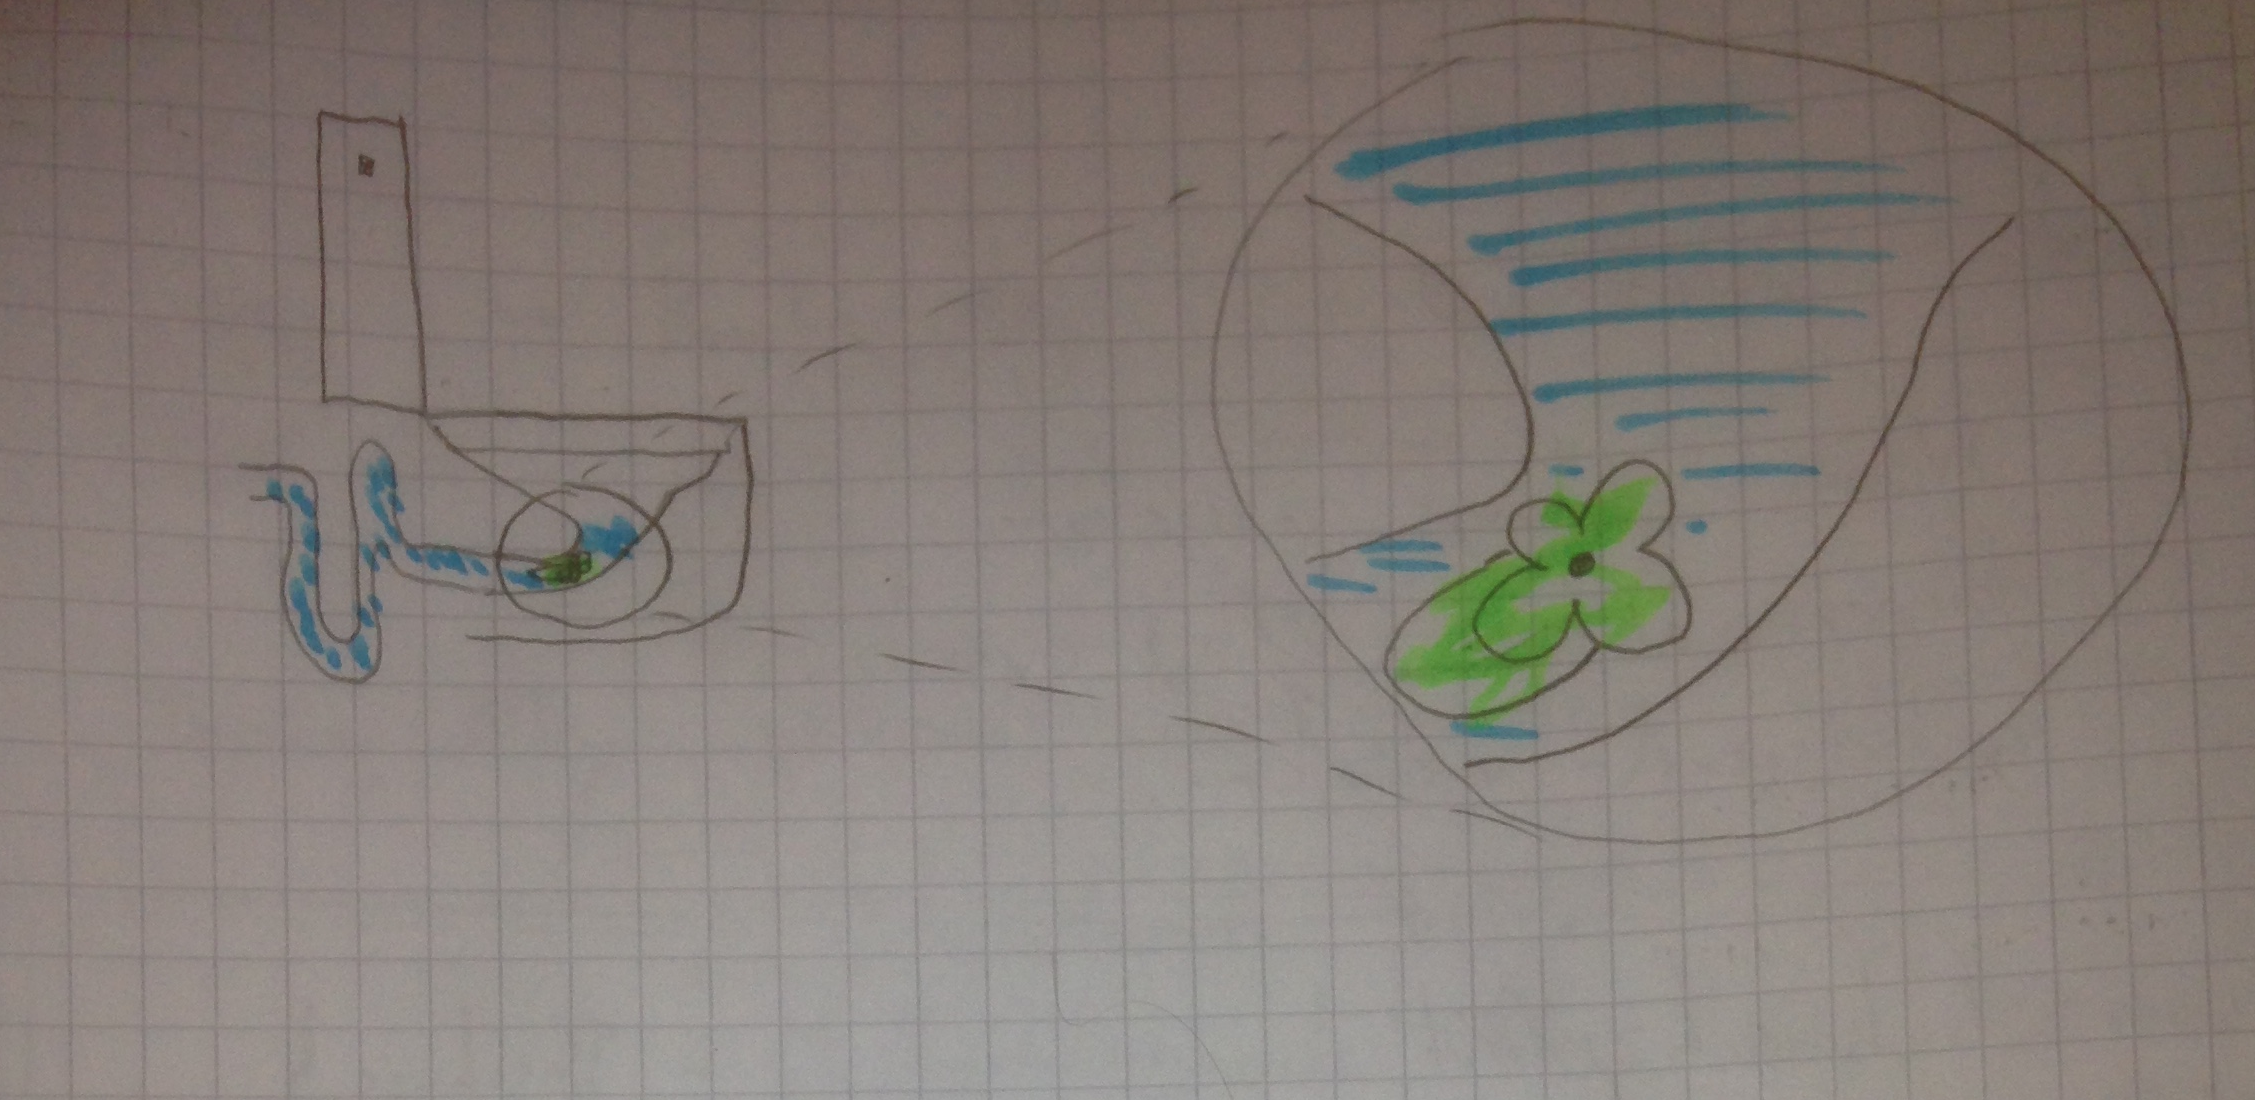
\includegraphics[scale=0.15]{bilder/durchfluss}
	\caption{Durchflusssensor}
	\label{fig:durchfluss}
\end{figure}

\subsection{Taster}
\label{ssec:taster}

Der Sensor wird auf den Taster der Toilette geklebt und ermittelt den Tastendruck kapazitiv.

\begin{figure}[H]
	\centering
	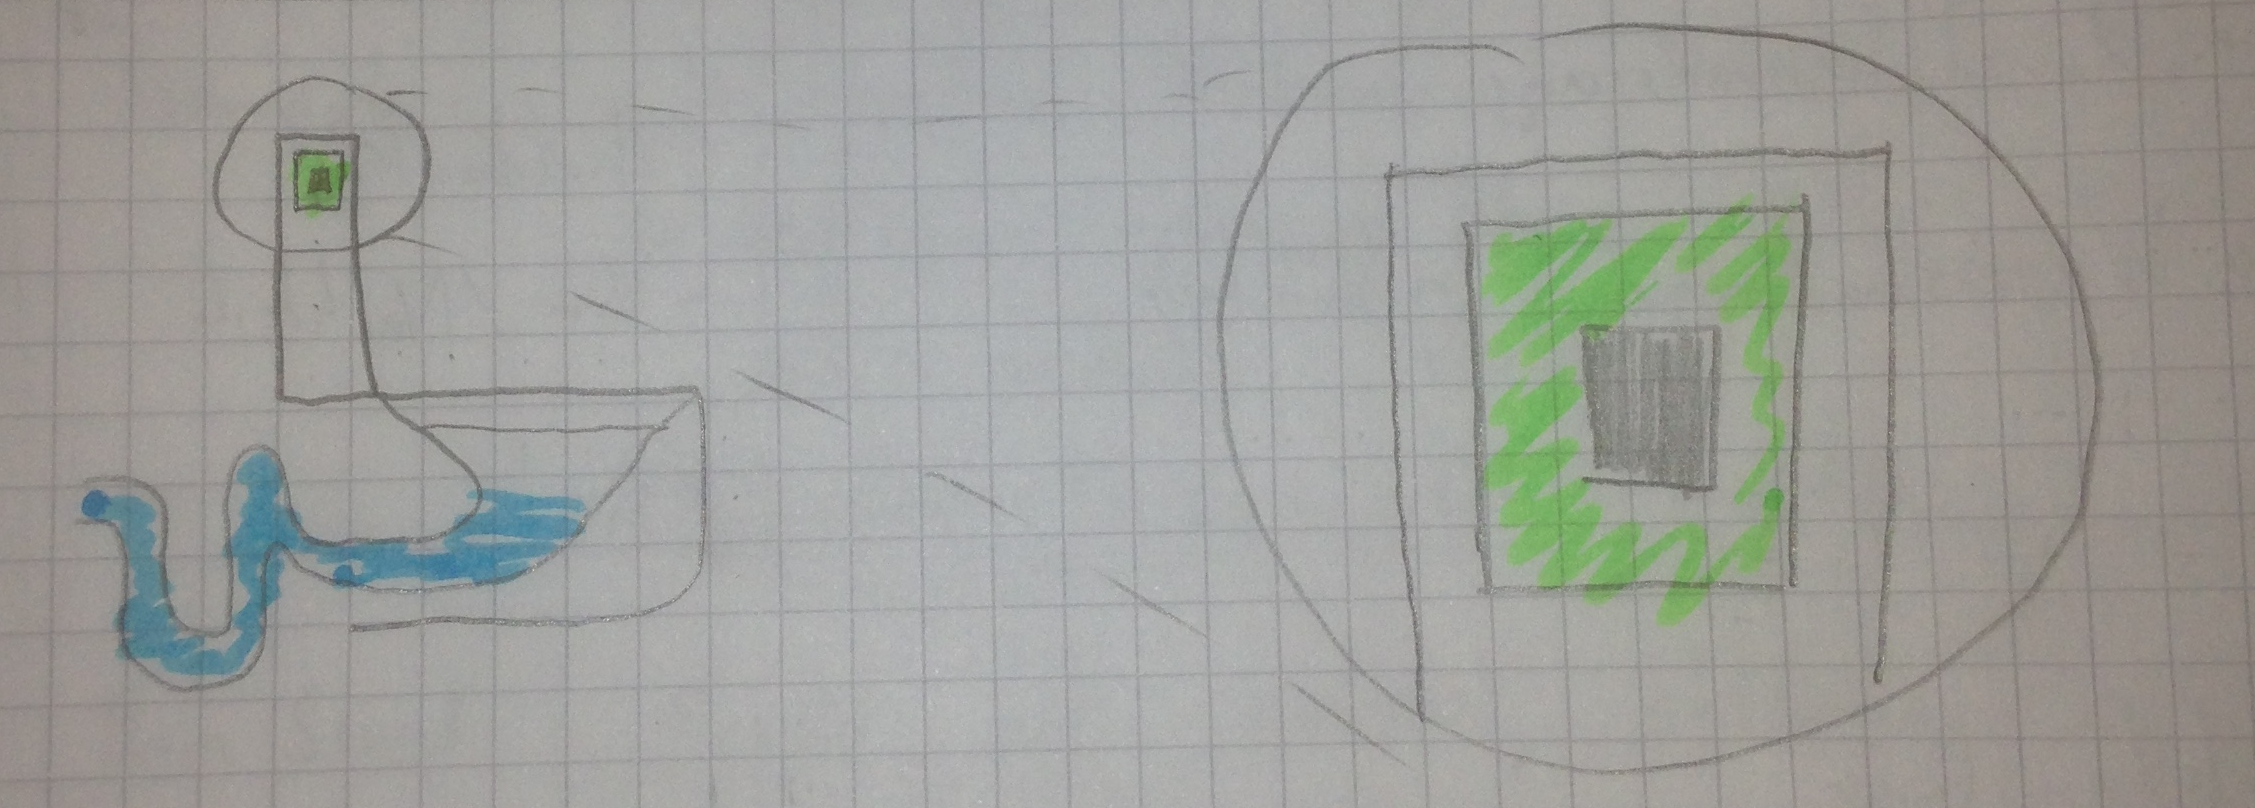
\includegraphics[scale=0.15]{bilder/taster}
	\caption{Kapazitiver Taster}
	\label{fig:taster}
\end{figure}

\subsection{Akustisch}
\label{ssec:taster}

Der Sensor wird an die Sch�ssel geklebt und misst �ber ein Mikrofon das Rauschen des Sp�lvorganges.

\begin{figure}[H]
	\centering
	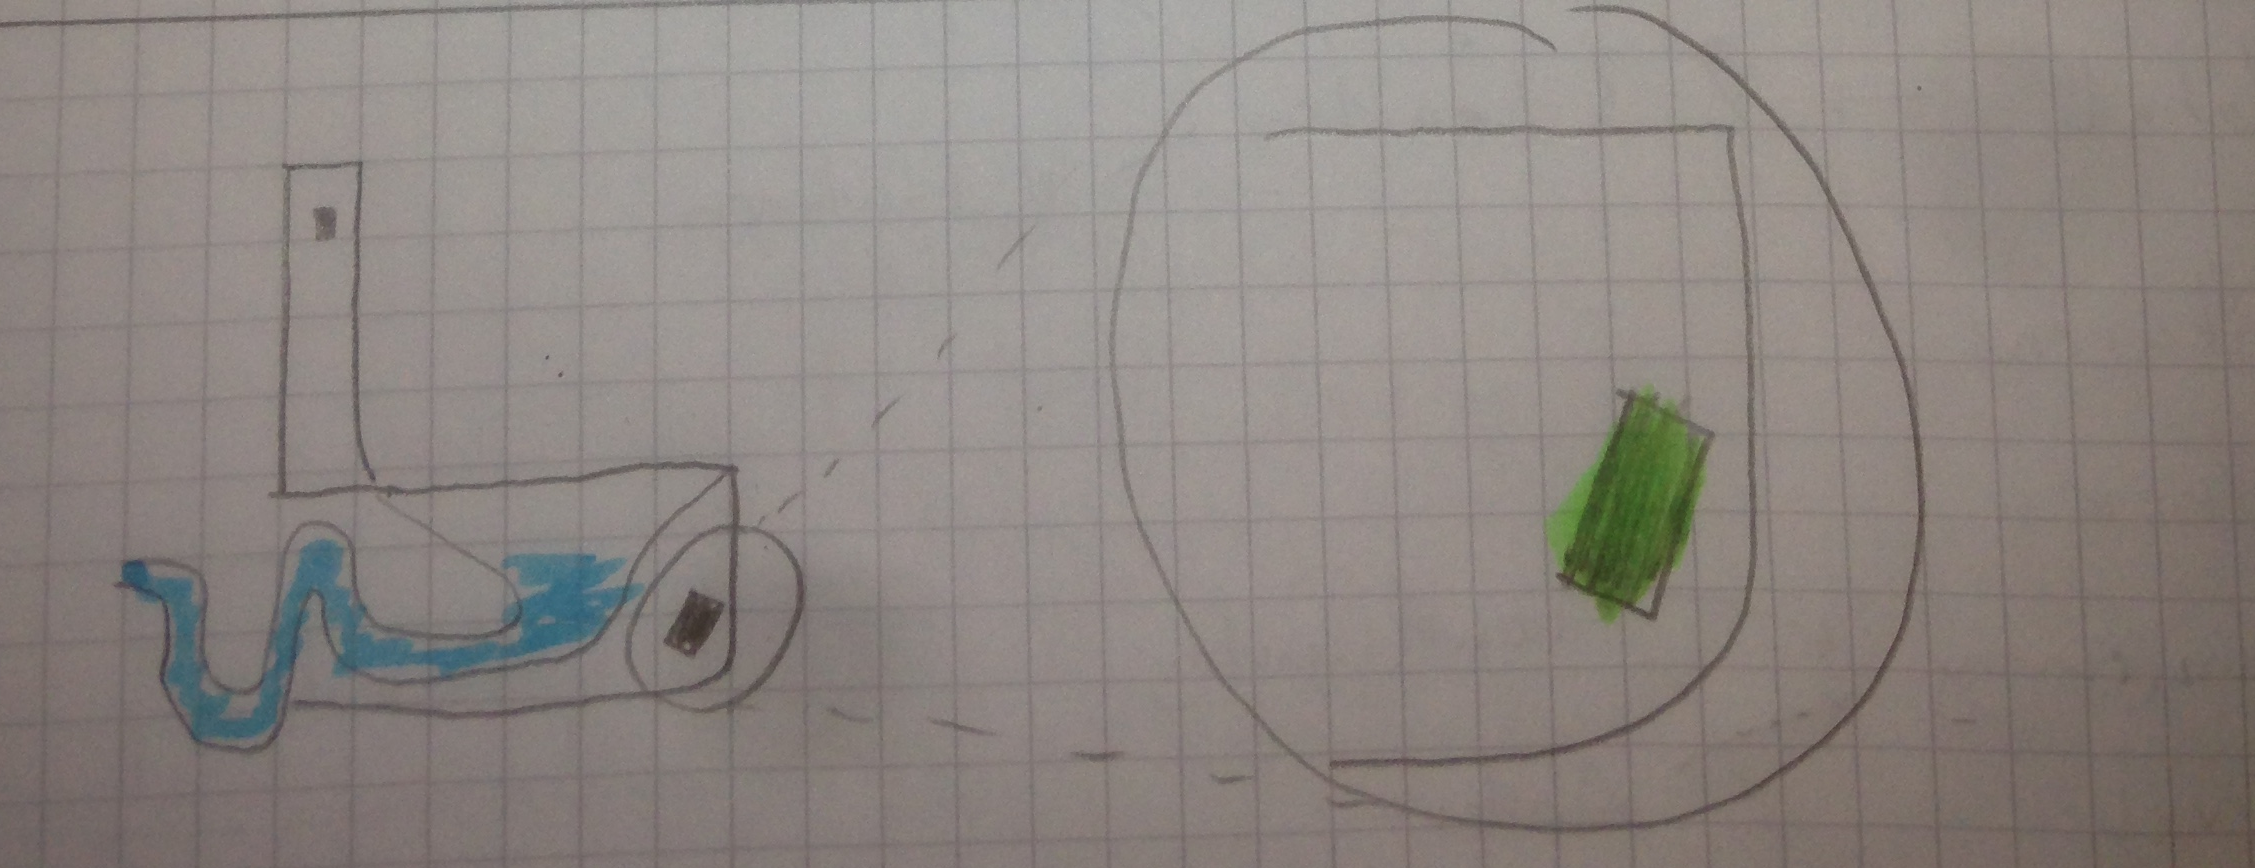
\includegraphics[scale=0.15]{bilder/akustisch}
	\caption{Akustisch}
	\label{fig:akustisch}
\end{figure}

\subsection{Gegen�berstellung}
\label{ssec:gegen�berstellung}

In der Gegen�berstellung vergeben wir f�r verschiedene Kriterien die Punkte: \\
\begin{equation}
0 \dots 3
\begin{cases}
-1,	& \text{Unpassend, kompliziert, umst�ndlich}  \\
0,  & \text{Neutral} \\
1,  & \text{Optimal, ideal, sehr einfach} \\
\end{cases}
\end{equation}

\begin{table}[H]
	\centering
	\begin{tabular}{r|ccc}
		\centering
		\textbf{Kriterium} & Durchfluss & Taster & Akustisch \\ \midrule
		Installation & 1 & 1 & 1\\
		Deinstallation & -1 & 0 & 1\\
		Stromverbrauch & 1 & 1 & 0\\
		Verschleiss & -1 & 0 & 1 \\
		Hygiene & 0 & 0 & -1\\
		Handhabung & 0 & 0 & 0\\
		Komplexit�t Umsetzung & -1 & 0 & 1\\
		\midrule
		& -1 & 2 & 3 \\
	\end{tabular}
	\caption{Gegen�berstellung}
	\label{tab:gegenueberstellung}
\end{table}

